\section{Research Method}

%You need to describe briefly the life cycle model or research method that you used. You do not need to write about all of the different process models that you are aware of. Focus on the process model or research method that you have used. It is possible that you needed to adapt an existing method to suit your project; clearly identify what you used and how you adapted it for your needs.

\todo[inline]{Talk about lit review here}

For this project, a literature review was undertaken to assess the work completed by researchers in the fields of Fuzzy Entropy and image alignment methods to help better understand what has been investigated, and to gain a personal background understanding.

\subsection{Entropy}

In terms of Information Theory, the Merriam-Webster Dictionary defines Entropy to be \cite{def_entropy}:

\begin{quotation}
 \textit{Entropy (noun): the degree of disorder or uncertainty in a system}
\end{quotation}

Shannon entropy can be mathematically defined:

\begin{equation}
  H(X) = - \displaystyle\sum_{i=0}^{N}{p_i \log_2 p_i}
\end{equation}
\myequations{Shannon Entropy}

Where $p_i$ is the set of probabilities for all the variables in $X$.

Let us consider a fair coin toss. The probability of heads is exactly $\frac{1}{2}$, therefore, the entropy of landing on heads is:

\begin{equation}
  \begin{split}
    H(heads) &= -\frac{1}{2}\log_2(\frac{1}{2}) - \frac{1}{2}\log_2(\frac{1}{2}) \\
    &= 1.0
  \end{split}
\end{equation}
\myequations{Shannon Entropy example - coin toss}

On the other side, if a system outputs solely the letter \say{M}, then the entropy of receiving the letter \say{M} is exactly 0. This is because when either the positive or the negative outcome is 100\%, then both sides equal \say{0} when fed into the entropy equation.
%http://mirror.ox.ac.uk/sites/ctan.org/graphics/pgf/contrib/pgfplots/doc/pgfplots.pdf
\begin{figure}[H]
\begin{center}
\pgfplotsset{every axis/.append style={thick},width=0.4*\textwidth, ymax=1}
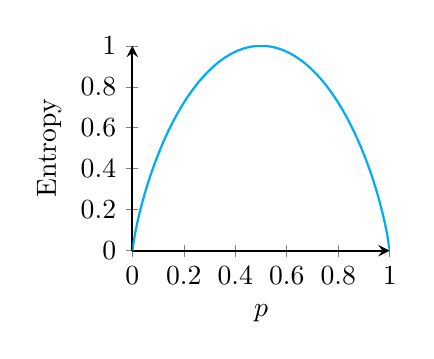
\begin{tikzpicture}
  \begin{axis}[
    axis lines = left,
    xlabel = $p$,
    ylabel = {Entropy},
    ]
  \addplot [
    domain=-0:1,
    samples=100,
    color=cyan,
    ]
    { -( x * log2(x) + (1-x) * log2(1-x) )};
  \end{axis}
\end{tikzpicture}
\end{center}
\caption{Entropy mapped against probability ($p$) of occurrence.}
\label{fig:entropy}
\end{figure}

\subsection{Uncertainty}

A certain amount of uncertainty in life is to be expected and sometimes desired. A surprise party for many is the nice kind of uncertainty, however uncertainty associated with risk - i.e. \say{Will I lose my job in the recession?} - is uncertainty with a negative impact. Modeling uncertainty is especially important so as researchers we can understand it, and use it to our advantage in techniques such as Fuzzy Entropy.

\subsubsection{Probabilistic Uncertainty}

By definition:

\begin{quotation}
  \textit{Probability: the chance that something will happen \cite{PROBABILITY}}
\end{quotation}

Probabilistic distribution is a widely accepted and used technique for representing expert judgements of uncertainty \cite{O’Hagan_2011}. Early work carried out by DeGroot (1970) \cite{degroot2004optimal}, built upon that of Savage (1954) \cite{Savage_1954}, gave a simple layman's explanation:

\begin{quotation}
  \textit{For instance, if the person prefers decision A to B and B to C then they must also prefer A to C.}
\end{quotation}

\subsubsection{Possibilistic Uncertainty}

By definition:

\begin{quotation}
  \textit{Possibility: a chance that something might exist, happen, or be true : the state or fact of being possible \cite{POSSIBILITY}}
\end{quotation}

Possibilistic uncertainty (closely related to \say{fuzziness}) indicates the lack of information we hold about the possible outcome values from a system - a sort of ambiguity. Possibilistic uncertainty models the possible outcomes from a system, as estimated by a decision maker because it is possibly impossible to determine beforehand \cite{Untiedt_2010}. For example,

\subsubsection{Indiscernibility Uncertainty}

By definition:

\begin{quotation}
  \textit{Indiscernibility: the quality or state of being indiscernible \cite{INDISCERNIBILITY}}

  \textit{Indiscernible: impossible to see, hear, or know clearly \cite{INDISCERNIBLE}}
\end{quotation}


\subsection{Fuzzy Entropy}

Fuzzy entropy stems from combining standard Entropy with the practices of Fuzzy Set Theory. This introduces the idea of \say{Membership} to a category, where an object can belong to more than one category to a certain degree.

One common example of this is listing someone as `Short', `Average' or `Tall' in height. If a tall person is someone over 6 feet in height, would a person who measured 5foot 11inches not be classified as tall? Given crisp sets, then they would be classified as `Average'. In fuzzy set theory, they would be be a certain degree of tall, and a certain degree of average, with the highest membership likely to win out when categorising their height. Another example of this can be seen in Figure \ref{fig:fuzzy-sets}

\begin{figure}[H]
  \center
  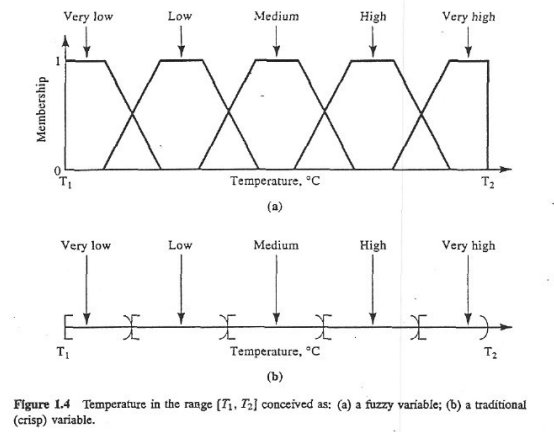
\includegraphics[scale=0.5]{/Users/lauracollins/Git/Major-Project/Documentation/Final/Chapter1/lit-review-img/fuzzy-sets.png}
  \caption{A comparison between Fuzzy Sets and Crisp sets. Image Source: Fuzzy Sets and Fuzzy Logic: Theory and Applications \cite{GEORGE_J_BO_2008}}
  \label{fig:fuzzy-sets}
\end{figure}

To combine Fuzzy Set Theory with Entropy, then the amount of fuzzy information gained from the fuzzy set(s) is known as Fuzzy Entropy.

\subsection{Joint Image Alignment}

Image Alignment focuses on the alignment of several images, into one average image.

\subsubsection{Learned-Miller`s Congealing}

Learned-Miller's Congealing \cite{joint-alignment} is often cited as being one of the first to truly align simple sets of data, with minimal noise, no occlusions and illumination variation \cite{Zhou_Lee_Yu_Efros_2015} \cite{peng2012rasl} \cite{Peng_Ganesh_Wright_Xu_Ma_2012}. Many more robust image alignment techniques have been developed off of the basis of this work, with more computational-expense.

This algorithm works by iteratively reducing the pixel-wise entropy over the input images, using a set of standard image transformations such as:

\begin{itemize}
  \item $x$ \& $y$ translations
  \item rotation
  \item $x$ \& $y$ sheer
  \item $x$ \& $y$ scale
\end{itemize}

The entropy is calculated by assessing each individual set of pixel-locations in the `Pixel Stack' (see Figure \ref{fig:pixel-stack}), and by calculating the entropy of the empirical distribution of values in the Pixel Stack.

\begin{figure}[H]
  \center
  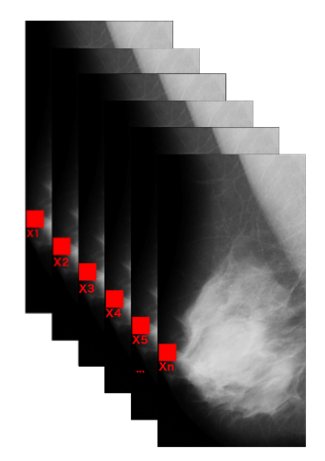
\includegraphics[scale=0.5]{/Users/lauracollins/Git/Major-Project/Documentation/Final/Chapter1/lit-review-img/pixels.png}
  \caption{Each pixel from the same location throughout the set creates a `Pixel Stack'}
  \label{fig:pixel-stack}
\end{figure}

As this project will be working with mammograms, something with little variation nor inconsistency, Congealing is the perfect, light-weight image alignment algorithm to which to build upon, especially as the demonstration code available for research has an entropy implementation already developed.

\subsubsection{Image Alignment using Fuzzy Entropy}

Some work has already been undertaken to investigate image alignment using Fuzzy Entropy metrics, however typically they are computationally costly, and therefore slow to run. This project will be investigating whether there are simpler, more light-weight fuzzy entropy metrics which could be implemented, for more everyday use in image alignment. It will also be investigated if, and further how, the outputs of these alignments differ per each fuzzy entropy metric.
